\documentclass{amsart}

\usepackage[utf8]{inputenc}
\usepackage[T2A]{fontenc}
\usepackage[english,russian]{babel}
\usepackage{amsthm,amsmath,amsfonts,amssymb}
\usepackage{fullpage}
\usepackage{eufrak}
\usepackage{bbm}

%%% Дополнительная работа с математикой
\usepackage{amsfonts,amssymb,amsthm,mathtools} % AMS
\usepackage{amsmath}
\usepackage{icomma}

%% Шрифты
\usepackage{euscript}	% Шрифт Евклид
\usepackage{mathrsfs}	% Красивый матшрифт

%% Свои команды
\DeclareMathOperator{\lb}{\mathop{lb}}	% логарифм по основанию 2
\DeclareMathOperator{\sgn}{\mathop{sgn}}	% сигнум
\renewcommand{\Im}{\mathop{\mathrm{Im}}\nolimits}	% мнимая часть
\renewcommand{\Re}{\mathop{\mathrm{Re}}\nolimits}	% вещественная часть
\renewcommand{\emptyset}{\varnothing}	% пустое множество
\renewcommand{\le}{\leqslant}	% отечественная версия "меньше или равно"
\renewcommand{\ge}{\geqslant}	% отечественная версия "больше или равно"
\renewcommand{\epsilon}{\varepsilon}	% стандартная "эпсилон"
\renewcommand{\phi}{\varphi}	% стандартная "фи"
\newcommand{\const}{\mathrm{const}}	% константа

%% Множества чисел
\DeclareMathOperator{\Natural}{\mathbb{N}}	% Натуральные числа
\DeclareMathOperator{\Integer}{\mathbb{Z}}	% Целые числа
\DeclareMathOperator{\Integerp}{\mathbb{Z}_{+}}	% Целые неотрицательные числа
\DeclareMathOperator{\Rational}{\mathbb{Q}}	% Рациональные числа
\DeclareMathOperator{\Real}{\mathbb{R}}	% Вещественные числа
\DeclareMathOperator{\Realp}{\mathbb{R}_{>0}}	% Вещественные положительные числа
\DeclareMathOperator{\Realn}{\mathbb{R}_{<0}}	% Вещественные отрицательные числа
\DeclareMathOperator{\Realnn}{\mathbb{R}_{\ge 0}}	% Вещественные неотрицательные числа
\DeclareMathOperator{\Realnp}{\mathbb{R}_{\le 0}}	% Вещественные неположительные числа
\DeclareMathOperator{\Complex}{\mathbb{C}}	% Комплексные числа

%% Заглавные греческие буквы
\DeclareMathOperator{\Alpha}{\mathrm{A}}	% Альфа
\DeclareMathOperator{\Beta}{\mathrm{B}}	% Вета
\DeclareMathOperator{\Epsilon}{\mathrm{E}}	% Эпсилон
\DeclareMathOperator{\Zeta}{\mathrm{Z}}	% Дзета
\DeclareMathOperator{\Eta}{\mathrm{H}}	% Эта
\DeclareMathOperator{\Iota}{\mathrm{I}}	% Йота
\DeclareMathOperator{\Kappa}{\mathrm{K}}	% Каппа
\DeclareMathOperator{\Mu}{\mathrm{M}}	% Мю
\DeclareMathOperator{\Nu}{\mathrm{N}}	% Ню
\DeclareMathOperator{\Omicron}{\mathrm{O}}	% Омикрон
\DeclareMathOperator{\Rho}{\mathrm{P}}	% Ро
\DeclareMathOperator{\Tau}{\mathrm{T}}	% Тау
\DeclareMathOperator{\Chi}{\mathrm{X}}	% Хи

%% Теория вероятностей
\renewcommand{\Prob}{\mathbb P}	% вероятность
\newcommand{\Expect}{\mathbb E}	% математическое ожидание
\renewcommand{\Variance}{\mathbb D}	% дисперсия
\newcommand{\Entropy}{\mathbb H}	% энтропия
\DeclareMathOperator{\cov}{\mathop{cov}}	% ковариация
\DeclareMathOperator{\supp}{\mathop{supp}}	% носитель
\DeclareMathOperator{\Skewness}{\mathop{Skew}}	% коэффициент асимметрии
\DeclareMathOperator{\Kurtosis}{\mathop{Kurt}}	% коэффициент эксцесса

%%% Статистический анализ
\newcommand*{\moment}[1]{\overline{#1}}	% выборочный момент
\DeclareMathOperator{\hskew}{\mathop{\widehat{Skew}}}	% выборочный коэффициент асимметрии
\DeclareMathOperator{\hkurt}{\mathop{\widehat{Kurt}}}	% выборочный коэффициент эксцесса
%% Однопараметрические распределения
\newcommand*{\chisq}[1]{\chi^2_{#1}}	% Распределение хи-квадрат
\newcommand*{\Stud}[1]{\mathcal{S}_{#1}}	% Распределение Стьюдента
\newcommand*{\Exp}[1]{\mathop{\mathrm{Exp}}(#1)}	% Показательное распределение
\newcommand*{\Bern}[1]{\mathop{\mathrm{Bern}}(#1)}	% Распределение Бернулли
\newcommand*{\Geom}[1]{\mathop{\mathrm{Geom}}(#1)}	% Геометрическое распределение
\newcommand*{\Pois}[1]{\mathop{\mathrm{Pois}}(#1)}	% Распределение Пуассона
%% Двухпараметрические распределения
\newcommand*{\FS}[2]{\mathcal{F}_{#1, #2}}	% Распределение Фишера-Снедекора
\newcommand*{\Norm}[2]{\mathcal{N}(#1, #2)}	% Нормальное распределение
\newcommand*{\Unif}[2]{\mathcal{U}(#1, #2)}	% Равномерное распределение
\newcommand*{\DE}[2]{\mathop{\mathrm{DE}}(#1, #2)}	% Распределение Лапласа
\newcommand*{\Cauchy}[2]{\mathop{\mathrm{C}}(#1, #2)}	% Распределение Коши
\newcommand*{\Binom}[2]{\mathop{\mathrm{Binom}}(#1, #2)}	% Биномиальное распределение
\newcommand*{\Betadist}[2]{\mathop{\mathrm{Beta}}(#1, #2)}	% Бета-распределение
\newcommand*{\Gammadist}[2]{\mathop{\mathrm{Gamma}}(#1, #2)}	% Гамма-распределение
%% Ажурные и готические буквы
\newcommand*{\Acl}{\mathcal{A}}	% A красивое
\newcommand*{\Ccl}{\mathcal{C}}	% C красивое
\newcommand*{\Fcl}{\mathcal{F}}	% F красивое
\newcommand*{\Icl}{\mathcal{I}}	% I красивое
\newcommand*{\Kcl}{\mathcal{K}}	% K красивое
\newcommand*{\Pcl}{\mathcal{P}}	% P красивое
\newcommand*{\Ycl}{\mathcal{Y}}	% Y красивое
\newcommand*{\Afr}{\mathfrak{A}}	% A готическое
\newcommand*{\Bfr}{\mathfrak{B}}	% B готическое
\newcommand*{\Ffr}{\mathfrak{F}}	% F готическое
\newcommand*{\Kfr}{\mathfrak{K}}	% K готическое
\newcommand*{\Xfr}{\mathfrak{X}}	% X готическое
%% Теория оценивания
\newcommand*{\ind}[1]{\mathbbm{1}_{\lbrace #1 \rbrace}}	% индикаторная функция
\newcommand*{\bias}[2]{\mathop{\mathrm{bias}}\nolimits_{#1}(#2)}	% смещение

%% Перенос знаков в формулах (по Львовскому)
\newcommand*{\hm}[1]{#1\nobreak\discretionary{}
	{\hbox{$\mathsurround=0pt #1$}}{}}

%%% Работа с картинками
\usepackage{graphicx,xcolor}	% Для вставки рисунков
\graphicspath{{images/}{images2/}}	% папки с картинками
\setlength\fboxsep{3pt}	% Отступ рамки \fbox{} от рисунка
\setlength\fboxrule{1pt}	% Толщина линий рамки \fbox{}
\usepackage{wrapfig}	% Обтекание рисунков и таблиц текстом
\RequirePackage{caption}
\DeclareCaptionLabelSeparator{defffis}{ "--- }
\captionsetup{justification=centering,labelsep=defffis}
\usepackage{float}
\usepackage{tikz}
\usepackage{pgfplots}
\pgfplotsset{compat=newest}
\usetikzlibrary{patterns}
\usetikzlibrary{calc}

%%% Работа с таблицами
\usepackage{array,tabularx,tabulary,booktabs}	% Дополнительная работа с таблицами
\usepackage{longtable}	% Длинные таблицы
\usepackage{multirow}	% Слияние строк в таблице
\usepackage{makecell}
\usepackage{multicol}


\renewcommand{\qedsymbol}{}

\newtheorem{problem}{Задание}

\begin{document}
	\newcommand{\problemset}[1]{
		\begin{center}
			\Large #1
		\end{center}
	}

	\begin{tabbing}
	\hspace{11cm} \= Студент: \= Божко-Домбровский Тимофей \\																			
	\> Группа: \> 2375 \\
	\> Вариант: \> 5 \\	
	\> Дата: \> \today
\end{tabbing}
\hrule
\vspace{1cm}	% файл с заголовком
	\problemset{Теория вероятностей и математическая статистика}
\problemset{Индивидуальное домашнее задание №1}

% Команда ниже задает "название" или слово, которое будет
% отображаться вместо proof или "доказательство"
% поскольку у нас в ИДЗ задачи - то нужно слово "Решение"
\renewcommand*{\proofname}{Решение}

%%%%%%%%%%%%%% ЗАДАНИЕ №1 %%%%%%%%%%%%%%
%% Условие задания №1
\begin{problem}
Из 35 книг, среди которых трехтомник А.С.Пушкина, выбирается наугад 18 и выставляется на полку. Определить вероятность того, что все три книги тома попадут на полку.\\
\end{problem}

%% Решение задания №1
\begin{proof}
Для начала определим множество исходов $\Omega$. Ясно, что в данном случае элементарным событием будет $ \omega_i $ = \{"данные 18 книг (из 35) выставлены на полку"\}. То есть $ \omega_i $ есть конкретное сочетание 18 книг из 35.\\Тогда очевидно, что:
\[ \#\Omega = \binom{35}{18} = \frac{35!}{18!\cdot\left(35-18\right)!} \]
Теперь определим событие $ A $. Подходят все элементарные события (сочетания 18 книг из 35), которые включают в себя книги трехтомника. А таких всего:
\[  \#A = \binom{3}{3}\cdot\binom{32}{15} = \frac{32!}{15!\cdot\left(32-15\right)!} \]

(тут учли, что были точно выбраны книги трехтомника и еще некоторые из оставшихся 32 книг)

Отсюда получаем, что вероятность наступления события $ A $ равна:
\[\frac{\#A}{\#\Omega} = \frac{32!}{15!\cdot17!}\cdot\frac{18!\cdot17!}{35!} = \frac{48}{385} \approx 0.1247 \]

{\it Ответ:} 0.1247
\end{proof}

%%%%%%%%%%%%%% ЗАДАНИЕ №2 %%%%%%%%%%%%%%
%% Условие задания №2
\begin{problem}
Прямые разбивают плоскость на полосы ширины 8. Определить вероятность того, то отрезок длинны 3, наугад брошенный на плоскость, не пересечет ни одной прямой.\\
\end{problem}

%% Решение задания №2
\begin{proof}
Ясно, что данная вероятностная задача относится к разделу задач на геометрическое определение вероятности. 
Одним из ограничений геометрического определения вероятности является условие, накладываемое на множество исходов $ \Omega $. Хоть само множество бесконечно большое (его мощность бесконечна), но мера $ V_d $ множества $ \Omega $ в пространсве $ \Real^d$ конечна.

В условии задачи же под $ \Omega $ автор понимает всю плоскость, а её мера $ V_2 $ в пространсве $ \Real^2 $ бесконечна. Мы получили некорректную формулировку вероятностной задачи.

Попробуем переформулировать задачу.
Неважно, в какую именно часть плоскости будет брошен отрезок, он всегда попадет как минимум на одну полосу (поскольку полос бесконечно много). Причем неважно, на какую именно полосу попал отрезок, полосы одинаковые, плоскость в любой части выглядит одинаково. 

Это значит, что достаточно рассмотреть в качестве $ \Omega $ лишь одну полосу ширины 8, вероятность того, что отрезок пересечет эту полосу и будет являться искомой вероятностью.

При этом не важно, что ширина полосы равна 8, а длинна бесконечна, ведь полоса в любой части относительно длинны выглядит одинаково, неважно, упал отрезок ниже или выше, он все равно упал на полосу.

Нарисуем картинку для решения задачи (см. рис.1).
\begin{figure}
    \centering
    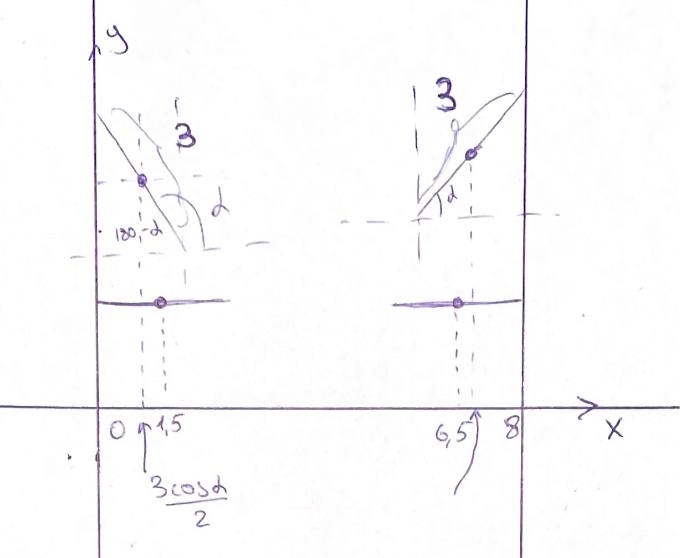
\includegraphics[width=0.5\linewidth]{1.jpg}
    \caption{}
    \label{fig:enter-label}
\end{figure}

Пусть $ x $ - это положение центра отрезка, а $ \alpha $ - угол между осью $ X $ и отрезком.\\
$ A =$ \{"отрезок не пересек ни одной прямой"\} - событие, вероятность которого нужно найти.\\
Соответственно $ 0\le x\le8 $ и $ 0\le\alpha\le\pi$.
Понятно, что при $ 1,5\le x\le6,5 $ угол может быть любым, а вот для остальных участков интервала на $ x $ и $ \alpha $ накладываются ограничения. Из рисунка видно, что чтобы отрезок не пересек прямую, нужно, чтобы:
\[
\begin{cases}
    x\ge\frac{3}{2}\cos{\alpha} 1.5, & \mbox{если } 0\le x < 1,5 \\
    x\le 8 - \frac{3}{2}\cos{\alpha}, & \mbox{если } 6,5 < x\le 8
\end{cases}
\]

Изобразим множества $ A $ и $ \Omega $ (см. рис.2).
\begin{figure}
    \centering
    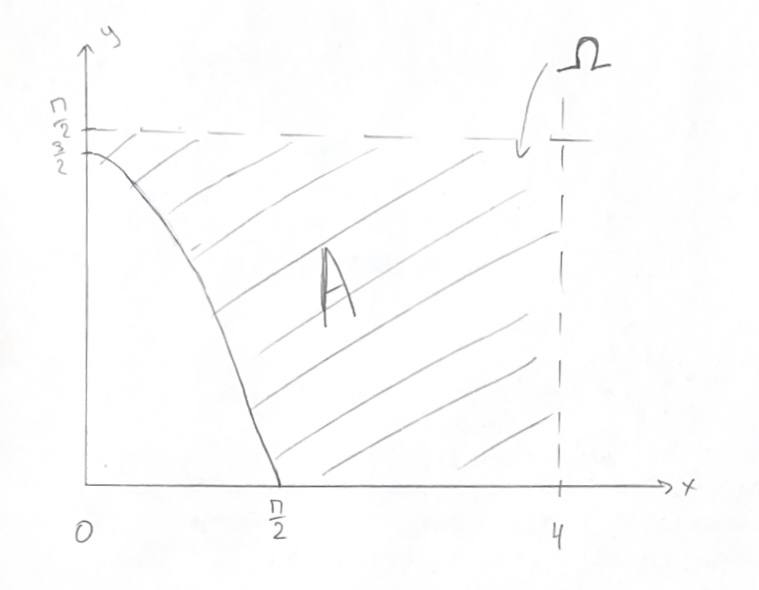
\includegraphics[width=0.5\linewidth]{2.jpg}
    \caption{}
    \label{fig:enter-label}
\end{figure}
Очевидно, что $ V_2\left(\Omega\right) = 8\pi$.\\
А вот меру $ A $ найдем вычитанием из меры (площади) $ \Omega $ мер (площадей) незаштрихованных уголков. Они, кстати, симметричны и площадь одного такого уголка можно найти как:

\[
\int\limits_0^{\pi/2} \frac{3}{2}\cos{\alpha} \, d\alpha = 1,5
\]
Тогда $ V_2\left(A\right) = 8\pi - 2\cdot 1,5 = 8\pi - 3$

Используя определение геометрической вероятности, находим, что:
\[
\Prob\left(A\right) = \frac{V_2\left(A\right)}{V_2\left(\Omega\right)} = \frac{8\pi - 3}{8\pi} = 1 - \frac{3}{8\pi} \approx 0.8806
\]
{\it Ответ:} 0.8806
\end{proof}

%%%%%%%%%%%%%% ЗАДАНИЕ №3 %%%%%%%%%%%%%%
%% Условие задания №3
\begin{problem}
В первой урне находится 8 белых и 8 красных шаров; во второй - 8 белых и 10 красных шаров; в третьей - 18 белых и 10 красных шаров. Наугад выбирают одну урну. Из неё достали 2 шара. Все оказались белыми. Определить вероятность того, что они из первой урны.\\
\end{problem}

%% Решение задания №3
\begin{proof}
Построим таблицу для определения ПГС.\\
Пусть $ H_1 $ = \{"Шары доставали из первой урны"\}. $ H_2 $ = \{"Шары доставали из второй урны"\}. $ H_3 $ = \{"Шары доставали из третьей урны"\}.\\
Событие $ A $ = \{"Из урны достали два белых шара"\}.\\
В итоге найти нам нужно вероятность $ H_1 $ при условии события $ A $.
\begin{center}
\begin{tabular}{ |c|c|c|c|c| } 
    \hline
    - & $ H_1 $ & $ H_2 $ & $ H_3 $ & $ \sum $\\ 
    \hline
    $\Prob\left(H_i\right)$ & $\frac{1}{3}$ & $\frac{1}{3}$ & $\frac{1}{3}$ & 1\\ 
    \hline
    $\Prob\left(A|H_i\right)$ & $\frac{8}{16}\cdot\frac{7}{15}$ & $\frac{8}{18}\cdot\frac{7}{17}$ & $\frac{18}{28}\cdot\frac{17}{27}$ & - \\ 
    \hline
\end{tabular}
\end{center}
Найдем вероятность события $ A $, используя формулу полной вероятности:
\[
\Prob\left(A\right) = \sum_{i=1}^3 \Prob\left(A|H_i\right)\cdot\Prob\left(H_i\right) = \frac{8}{16}\cdot\frac{7}{15}\cdot\frac{1}{3} + \frac{8}{18}\cdot\frac{7}{17}\cdot\frac{1}{3} + \frac{18}{28}\cdot\frac{17}{27}\cdot\frac{1}{3} = \frac{4397}{16065}
\]
Найдем вероятность $ H_1 $ используя формулу Байеса:
\[
\Prob\left(H_1|A\right) = \frac{\Prob\left(A|H_1\right)\cdot\Prob\left(H_1\right)}{\Prob\left(A\right)} = \frac{\frac{7}{30}\cdot\frac{1}{3}}{\frac{4397}{16065}} = \frac{2499}{8794} \approx 0.2842
\]
{\it Ответ:} 0.2842
\end{proof}

%%%%%%%%%%%%%% ЗАДАНИЕ №4 %%%%%%%%%%%%%%
%% Условие задания №4
\begin{problem}
Электростанция находится в городе А, из которого проведены ЛЭП в посёлки В и С. Кроме того посёлки В и С соеденены ЛЭП между собой и с посёлком D каждый. В результате урагана вероятность повреждения линий AB и AC равна 0.5, а линий BC, BD и CD - 0.3. Определить вероятность того, что электроснабжение посёлка D не будет нарушено.
\end{problem}

%% Решение задания №4
\begin{proof}
Для решения задачи нарисуем рисунок (см. рис.3).
\begin{figure}
    \centering
    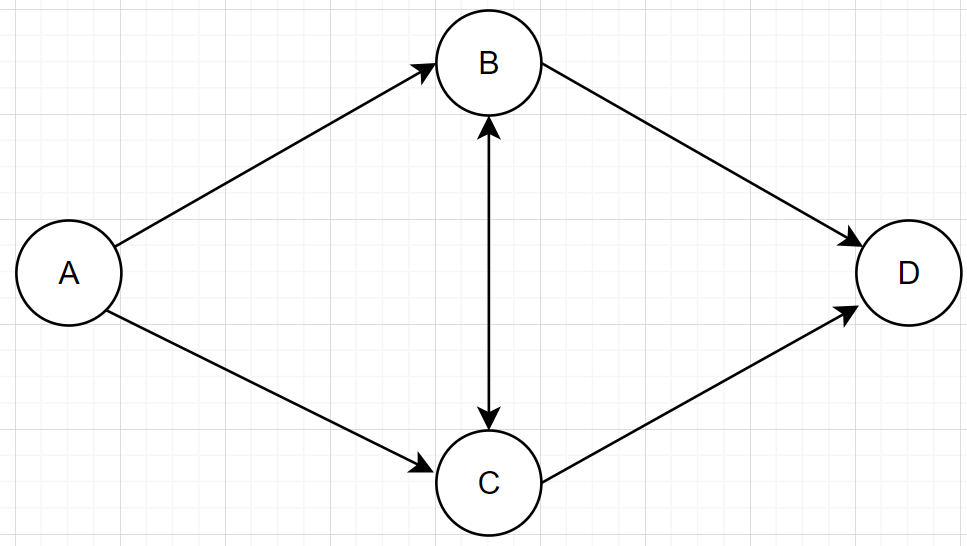
\includegraphics[width=0.5\linewidth]{3.png}
    \caption{}
    \label{fig:enter-label}
\end{figure}

Пусть событие $ A = $ \{"Электроснабжение посёлка D не будет нарушено"\}. Тогда, событие $ \neg A = $ \{"Электроснабжение посёлка D будет нарушено"\}. Понятно, что легче всего посчитать вероятность события $ \neg A $, тогда вероятность события $ A $ найдется как:
\[
\Prob\left(A\right) = 1 - \Prob\left(\neg A\right)
\]

Электроснабжение будет нарушено в четырех случаях:\\
1) Повредились линии AB и AC\\
2) Повредились линии BD и CD\\
3) Повредились линии AC, BC и BD\\
4) Повредились линии AВ, BC и СD\\
Любой из этих случаев приводит к нарушению электроснабжения.
То есть:
\[
\Prob\left(\neg A\right) = \Prob\left(1\cup 2\cup 3\cup 4\right) = \Prob\left(1\right) + \Prob\left(2\right) + \Prob\left(3\right) + \Prob\left(4\right)
\]
Где:
\begin{gather*}
    \Prob\left(1\right) = \Prob\left(AB\cap AC\right) = \Prob\left(AB\right)\cdot\Prob\left(AC\right) = 0.5\cdot 0.5 = 0.25\\
    \Prob\left(2\right) = \Prob\left(BD\cap CD\right) = \Prob\left(BD\right)\cdot\Prob\left(CD\right) = 0.3\cdot 0.3 = 0.09\\
    \Prob\left(3\right) = \Prob\left(AC\cap BC\cap BD\right) = \Prob\left(AC\right)\cdot\Prob\left(BC\right)\cdot\Prob\left(BD\right) = 0.5\cdot 0.3\cdot 0.3 = 0.045\\
    \Prob\left(4\right) = \Prob\left(AB\cap BC\cap CD\right) = \Prob\left(AB\right)\cdot\Prob\left(BC\right)\cdot\Prob\left(CD\right) = 0.5\cdot 0.3\cdot 0.3 = 0.045
\end{gather*}
Тут учли, что события \{"повреждена линия X"\} и \{"повреждена линия Y"\} независимые, следовательно вероятность их пересечения равна произведению вероятностей каждого из событий.
Итого $ \Prob\left(\neg A\right) = 0.25 + 0.09 + 0.045 + 0.045 = 0.43 $\\
Тогда $ \Prob\left(A\right) = 1 - \Prob\left(\neg A\right) = 1 - 0.43 = 0.57$

{\it Ответ:} 0.57
\end{proof}

%%%%%%%%%%%%%% ЗАДАНИЕ №5 %%%%%%%%%%%%%%
%% Условие задания №5
\begin{problem}
Вероятность успеха в схеме берунли равна $ \frac{1}{5} $. Проводится 2000 испытаний. Написать точную формулу и вычислить приближённо вероятность того, что число успехов равно 382.
\end{problem}

%% Решение задания №5
\begin{proof}
Воспользуемся формулой $ \Prob\left(\mu_n = k\right) = \binom{n}{k}\cdot p^k\cdot\left(1-p\right)^{n-k} $\\
Тогда $ \Prob\left(\mu_{2000} = 382\right) = \binom{2000}{382}\cdot 0.2^{382}\cdot 0.8^{1618} $\\
Поскольку проводится большое число испытаний, посчитаем вероятность приближенно.
$ n\cdot p = 2000\cdot\frac{1}{5} = 400 > 10 \Rightarrow $ воспользуемся схемой Муавра-Лапласа:
\[
P_n\left(k\right) \approx \frac{1}{\sqrt{np(1-p)}}\cdot\varphi(X_{n,k})
\]
Где $ \varphi(x) = \frac{1}{\sqrt{2\pi}}\cdot\exp{\left(-\frac{x^2}{2}\right)} $ и $ X_{n,k} = \frac{k - np}{\sqrt{np(1-p)}} $.

\begin{gather*}
    X_{2000, 382} = \frac{382 - 2000\cdot 0.2}{\sqrt{2000\cdot 0.2\cdot 0.8}} \approx -1.00623 \\
    \varphi(X_{2000,382}) =  \frac{1}{\sqrt{2\pi}}\cdot\exp{\left(-\frac{(-1.00623)^2}{2}\right)} \approx 0.240463\\
    P_{2000}\left(382\right) \approx \frac{1}{\sqrt{2000\cdot 0.2\cdot 0.8}} \cdot 0.240463 \approx 0.0134423 \approx 0.0134
\end{gather*}

{\it Ответ:} 0.0134
\end{proof}	% файл с решениями
        %\problemset{Теория вероятностей и математическая статистика}
\problemset{Индивидуальное домашнее задание №0}	% поменяйте номер ИДЗ

\renewcommand*{\proofname}{Решение}

%%%%%%%%%%%%%% ЗАДАНИЕ №1 %%%%%%%%%%%%%%
%% Условие задания №1
\begin{problem}
	Из урны, в которой лежат $ K $ белых и $ L $ чёрных шаров, наудачу выбирают один шар. Чему равна вероятность того, что этот шар "--- белый?
\end{problem}

%% Решение задания №1
\begin{proof}
	Пусть $ A $ "--- событие, что достали белый шар.
	Количество всех исходов будет равно: $ \#\Omega \hm= K + L $.
	
	Тогда количество благоприятных исходов (наступления события $ A $) равно: $ \#A = K $.
	
	Отсюда получаем, что вероятность наступления события $ A $ равна:
	\[ \Prob A = \cfrac{\#A}{\#\Omega} = \cfrac{K}{K + L}. \]
\end{proof}

%%%%%%%%%%%%%% ЗАДАНИЕ №2 %%%%%%%%%%%%%%
%% Условие задания №2
\begin{problem}
	Распределение случайной величины $ \xi $ задано таблицей:
	\begin{center}
		\begin{tabular}{|c|c|c|c|c|c|}
		\hline
		$ \xi $ & 1 & 2 & 4 & 6 & $ \Sigma $ \\
		\hline
		$ \mathbb{P} $ & 0,1 & 0,2 & 0,6 & 0,1 & 1 \\
		\hline
		\end{tabular}
	\end{center}
	Вычислить $ \Expect\xi $, $ \Variance\xi $, $ \Entropy\xi $ (в натах) и распределение $ \eta = \sin(\pi\xi/3) $.
\end{problem}

%% Решение задания №2
\begin{proof}
	Математическое ожидание дискретной случайной величины $ \xi $ задаётся формулой:
	\[ \Expect\xi = \sum_{i \colon p_i > 0}a_ip_i. \]
	Отсюда получаем:
	\[ \Expect\xi = 1 \cdot 0,1 + 2 \cdot 0,2 + 4 \cdot 0,6 + 6 \cdot 0,1 = 3,5. \]
	Дисперсия дискретной случайной величины $ \xi $ задаётся формулой:
	\[ \Variance\xi = \sum_{i \colon p_i > 0}(a_i - \mathbb E\xi)^2p_i. \]
	Отсюда получаем:
	\[ \Variance\xi = (1 - 3,5)^2 \cdot 0,1 + (2 - 3,5)^2 \cdot 0,2 + (4 - 3,5)^2 \cdot 0,6 + (6 - 3,5)^2 \cdot 0,1 = 1,85. \]
	Энтропия дискретной случайной величины $ \xi $ задаётся формулой:
	\[ \Entropy\xi = -\sum_{i \colon p_i > 0}p_i\log_bp_i. \]
	Необходимо вычислить энтропию в натах, т~е. $ b = e $. Получим:
	\[ \Entropy\xi = -(0,1 \cdot \ln0,1 + 0,2 \cdot \ln0,2 + 0,6 \cdot \ln0,6 + 0,1 \cdot \ln0,1) \approx 1,0889. \]
	Носитель случайной величины $ \xi $ имеет вид: $ \supp \xi = \lbrace 1, 2, 4, 6 \rbrace $. Тогда носитель случайной величины $ \eta $ будет иметь вид: $ \supp \eta = \left\lbrace -\frac{\sqrt{3}}{2}, 0, \frac{\sqrt{3}}{2} \right\rbrace  $. Найдём вероятности появления каждого числа:
	\begin{align*}
		\Prob(\eta = -\sqrt{3}/2) &= \Prob(\xi = 4) = 0,6. \\
		\Prob(\eta = 0) &= \Prob(\xi = 6) = 0,1. \\
		\Prob(\eta = \sqrt{3}/2) &= \Prob(\xi = 1) + \Prob(\xi = 2) = 0,3.
	\end{align*}
	Таким образом, можно записать распределение случайной величины $ \eta $ в виде таблицы:
	\begin{center}
		\begin{tabular}{|c|c|c|c|c|}
			\hline
			$ \eta $  & $ -\sqrt{3}/2 $ & 0   & $ \sqrt{3}/2 $ & $ \Sigma $ \\ \hline
			$ \Prob $ & 0,6             & 0,1 & 0,3            & 1          \\ \hline
		\end{tabular}
	\end{center}
\end{proof}

%%%%%%%%%%%%%% ЗАДАНИЕ №3 %%%%%%%%%%%%%%
%% Условие задания №3
\begin{problem}
	Условие задачи №3.
\end{problem}

%% Решение задания №3
\begin{proof}
	Решение задачи №3.
\end{proof}
\end{document}